\chapter{Experiment Setup and Results}
\label{chap:results}

This chapter evaluates \textsc{StructPF} against one-shot generation across two studies to address our fourth research goal (G4, Sections~\ref{sec:res-setup} to~\ref{sec:res-grounding}), and then reports two negative results with simulated students that motivated grounding Stage~1 on curriculum data (Section~\ref{sec:res-negative-signals}).

\section{Experiment Setup}
\label{sec:res-setup}

We organize our main evaluation in two studies. First, Study~A evaluates how well \textsc{StructPF} as a whole builds the underlying PF structure compared with one-shot prompting under \textsc{PF Eval}, and validates the automated verdicts against blinded human ratings on a stratified sample of tasks. Second, because knowing what students can and cannot yet do is a core bottleneck in PF design, Study~B tests our Stage~1 design across 30 curriculum topics to see how well an LLM identifies the boundary of students' prior knowledge on its own and whether external curriculum grounding actually improves this bottleneck.

\subsection{Study A: \textsc{PF Eval} Setup}
\label{subsec:res-setup-a}

Study~A reuses the four Grade~7 settings from Chapter~\ref{chap:oneshot}, where each setting fixes the target concept and two earlier-grade prerequisite standards in advance, as shown in Figure~\ref{fig:res-setup-a}. We compare the 118 GPT-5 mini and 120 GPT-4.1 one-shot tasks from Chapter~\ref{chap:oneshot} against 120 tasks from \textsc{StructPF} with GPT-5 mini and Stage~1 fixed to the same prerequisites, and evaluate all 358 tasks with \textsc{PF Eval} in Sections~\ref{sec:res-oneshot} and~\ref{sec:res-progression}. To verify that \textsc{PF Eval} correlates with human judgment on generated tasks and to validate our framework as a whole, we also conduct a blinded human evaluation on a stratified sample of 24 tasks in Section~\ref{sec:res-human-eval}.

\begin{figure}[!htb]
    \centering
    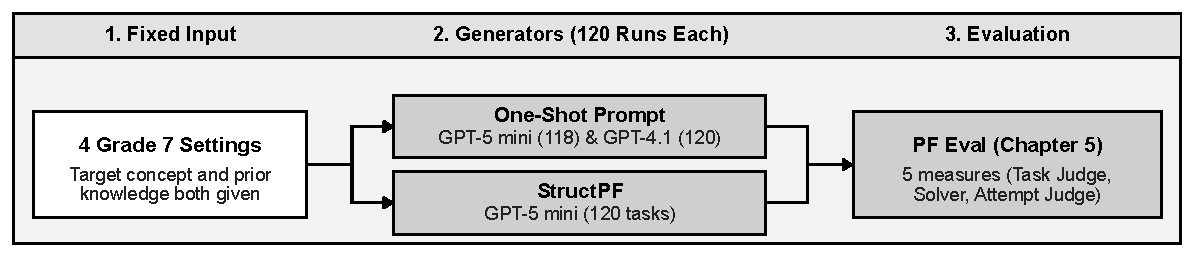
\includegraphics[width=0.92\textwidth]{figures/fig6_1_study_a_setup.pdf}
    \caption[Study A Setup: Four Grade 7 Settings with Fixed Prior Knowledge]{Study~A Setup: Four Grade~7 Settings with Fixed Prior Knowledge}
    \label{fig:res-setup-a}
\end{figure}

\subsection{Study B: Curriculum Grounding Setup}
\label{subsec:res-setup-b}

While Study~A provided the prerequisite standards in the setting as in Chapter~\ref{chap:oneshot}, Study~B gives only the target concept across 30 Common Core topics from Grades~5 to~10 and compares three GPT-5 mini generators with one task per topic, namely the one-shot prompt, \textsc{StructPF} without grounding where Stage~1 relies on the model alone, and \textsc{StructPF} with grounding where Stage~1 retrieves prerequisites from the Learning Commons graph, as shown in Figure~\ref{fig:res-setup-b}. Comparing the one-shot prompt with \textsc{StructPF} without grounding tests whether separating prior-knowledge identification into Stage~1 helps on its own, while comparing the two \textsc{StructPF} variants tests how much external curriculum data adds beyond the staged structure. In each run, the generator outputs both the student task and its proposed prior skills. Because a generator might list the target formula itself as prior knowledge, we evaluate each run with the Two-Step Check in Figure~\ref{fig:res-setup-b} using GPT 5.6 Luna, checking first whether the proposed prior skills stay within official prerequisites in the Prior-Knowledge Check and second whether those valid skills fall short on the task numbers in the Method-Failure Check.

\begin{figure}[!htb]
    \centering
    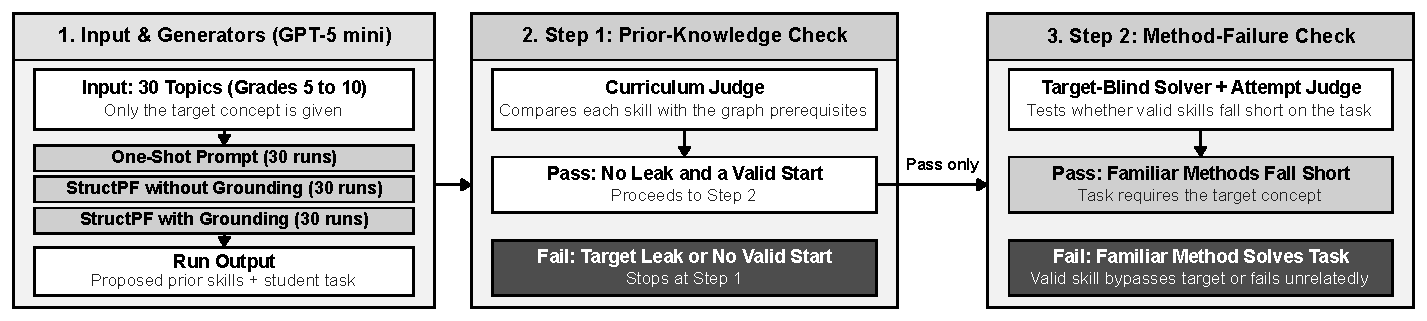
\includegraphics[width=\textwidth]{figures/fig6_2_study_b_setup.pdf}
    \caption[Study B Setup: Curriculum Topics and Two-Step Check]{Study~B Setup: Curriculum Topics and Two-Step Check}
    \label{fig:res-setup-b}
\end{figure}

\section{Study A: \textsc{PF Eval} Experiment Results}
\label{sec:res-study-a}

\subsection{One-Shot Tasks under \textsc{PF Eval}}
\label{sec:res-oneshot}

We first apply the five measures of \textsc{PF Eval} to the 238 ready one-shot tasks from Study~A to identify which PF requirement breaks down most often.

\begin{figure}[!htb]
    \centering
    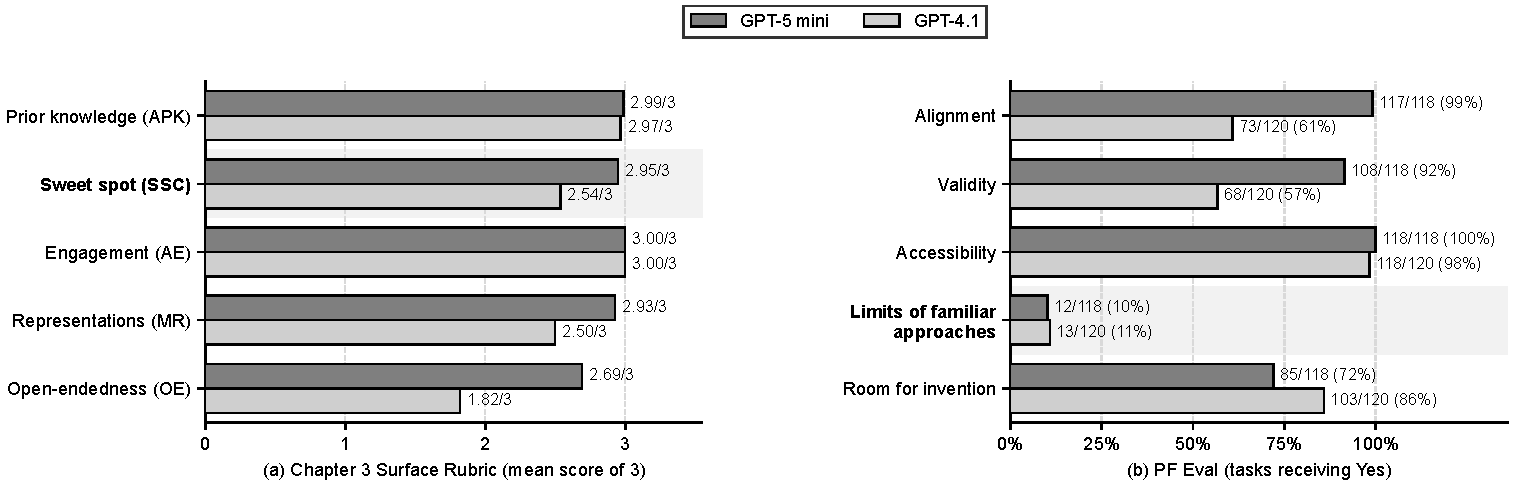
\includegraphics[width=\textwidth]{figures/fig6_3_oneshot_outcomes.pdf}
    \caption[Surface Rubric versus \textsc{PF Eval} on One-Shot Tasks]{Surface Rubric versus \textsc{PF Eval} on One-Shot Tasks}
    \label{fig:res-oneshot-outcomes}
\end{figure}

Figure~\ref{fig:res-oneshot-outcomes} compares the Chapter~\ref{chap:oneshot} surface rubric (Figure~\ref{fig:res-oneshot-outcomes}a) directly against \textsc{PF Eval} (Figure~\ref{fig:res-oneshot-outcomes}b) on the 238 one-shot tasks. Most tasks pass the soundness and accessibility checks, and on room for invention GPT-4.1 even overtakes GPT-5 mini ($86\%$ versus $72\%$), reversing the rubric's open-endedness scores ($1.82$ versus $2.69$ out of 3) because GPT-5 mini's multi-part worksheets narrow the student's procedure. The sharpest discrepancy is on whether familiar methods fall short. Whereas the surface rubric rates sweet spot calibration near the ceiling at $2.95$ and $2.54$ out of 3, testing the tasks with the solver shows that familiar methods fall short on only 12 of 118 GPT-5 mini tasks ($10\%$) and 13 of 120 GPT-4.1 tasks ($11\%$). Because a single prompt writes the story and chooses the numbers at once without verifying them, it almost always picks untied values that a familiar calculation such as a single average or unit rate settles right away.

\subsection{\textsc{StructPF} under \textsc{PF Eval}}
\label{sec:res-progression}

We next evaluate the 120 tasks generated by \textsc{StructPF} on the same four Grade~7 settings. In Table~\ref{tab:res-structpf-fixed}, the top rows compare \textsc{StructPF} with the two one-shot baselines, and the bottom rows break \textsc{StructPF} down by setting.

\begin{table}[!htb]
    \centering
    \caption[One-Shot Prompting versus \textsc{StructPF} on the Four Grade 7 Settings (Study A)]{One-Shot Prompting versus \textsc{StructPF} on the Four Grade~7 Settings (Study~A)}
    \label{tab:res-structpf-fixed}
    \footnotesize
    \setlength{\tabcolsep}{3.4pt}
    \begin{tabular}{@{}lcccccccc@{}}
        \toprule
        & & & \multicolumn{2}{c}{\textbf{Task Soundness}} & \multicolumn{4}{c}{\textbf{PF Requirements}} \\
        \cmidrule(lr){4-5} \cmidrule(l){6-9}
        \textbf{Generator / Setting} & \textbf{Ready} & \textbf{Rubric} & \textbf{Align.} & \textbf{Valid.} & \textbf{Access.} & \textbf{Limits} & \textbf{Invention} & \textbf{All 5} \\
        \midrule
        One-Shot (GPT-4.1) & 120 & 12.8 & 73 ($61\%$) & 68 ($57\%$) & 118 ($98\%$) & 13 ($10.8\%$) & 103 ($86\%$) & 4 ($3.3\%$) \\
        One-Shot (GPT-5 mini) & 118 & 14.6 & 117 ($99\%$) & 108 ($92\%$) & 118 ($100\%$) & 12 ($10.2\%$) & 85 ($72\%$) & 10 ($8.5\%$) \\
        \textsc{StructPF} (GPT-5 mini) & 120 & 12.1 & \textbf{120 ($100\%$)} & \textbf{114 ($95\%$)} & 117 ($98\%$) & \textbf{96 ($80.0\%$)} & \textbf{88 ($73\%$)} & \textbf{68 ($57\%$)} \\
        \midrule
        \quad Music distributions & 30 & 13.2 & 30 & 30 & 30 & 27 ($90.0\%$) & 28 ($93\%$) & 25 ($83\%$) \\
        \quad Composite garden area & 30 & 10.8 & 30 & 25 & 30 & 25 ($83.3\%$) & 23 ($77\%$) & 17 ($57\%$) \\
        \quad Basketball ratios & 30 & 12.3 & 30 & 29 & 30 & 23 ($76.7\%$) & 20 ($67\%$) & 15 ($50\%$) \\
        \quad Shopping discounts & 30 & 12.1 & 30 & 30 & 27 & 21 ($70.0\%$) & 17 ($57\%$) & 11 ($37\%$) \\
        \bottomrule
    \end{tabular}
\end{table}

As shown in Table~\ref{tab:res-structpf-fixed}, \textsc{StructPF} increases the share of tasks where familiar methods fall short nearly eightfold over one-shot GPT-5 mini, from 12 of 118 ($10.2\%$) to 96 of 120 ($80.0\%$), while keeping alignment ($100\%$), mathematical validity ($95\%$), accessibility ($98\%$), and room for invention ($73\%$) high. Across the four settings, familiar methods fall short on between $70.0\%$ of tasks in shopping discounts and $90.0\%$ in music distributions. Taken over all five measures, 68 of the 120 \textsc{StructPF} tasks ($57\%$) pass every measure, compared with 10 of 118 for one-shot GPT-5 mini ($8.5\%$) and 4 of 120 for one-shot GPT-4.1 ($3.3\%$). By contrast, the Chapter~\ref{chap:oneshot} surface rubric scores \textsc{StructPF} lower than one-shot GPT-5 mini at $12.1$ versus $14.6$ out of 15, because \textsc{StructPF} withholds the rubric from Stage~3 and fixes the quantities around a single comparison rather than listing multiple representations or sub-questions.

Figure~\ref{fig:res-structpf-examples} shows two of the 68 \textsc{StructPF} tasks that pass all five measures. In the basketball task, both drills score 20 points in 10 minutes, so the overall rate from Grade~6 cannot tell them apart, and students have to discover that a proportional relationship needs the same rate in every segment. In the shopping task, adding the two discounts gives the same price at both stores, so students have to notice that the second discount applies to the already reduced price. In both tasks, the familiar method ends in a tie, while the task still leaves the key idea to the student.

\begin{figure}[!htb]
    \centering
    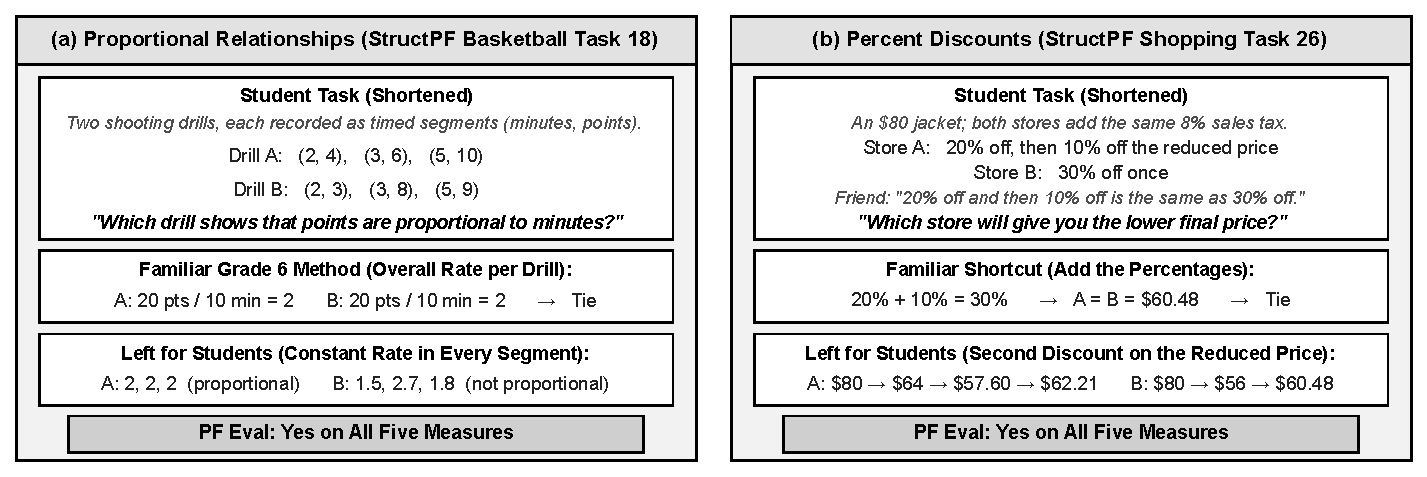
\includegraphics[width=\textwidth]{figures/fig6_5_structpf_examples.pdf}
    \caption[Two \textsc{StructPF} Tasks Passing All Five \textsc{PF Eval} Measures (Basketball and Shopping)]{Two \textsc{StructPF} Tasks Passing All Five \textsc{PF Eval} Measures (Basketball and Shopping)}
    \label{fig:res-structpf-examples}
\end{figure}

Although \textsc{StructPF} improves the PF requirements, it still misses a measure on some of the 120 tasks. Most of these misses come from two causes.

\begin{enumerate}[leftmargin=0.6cm,label=\textbf{\arabic*.},itemsep=0.6em,topsep=0.4em]
    \item \textbf{The Task Gives Away the Route (32 Tasks)}\\[0.2em]
    The task states the calculation route that students should find themselves, so room for invention fails. Shopping Task~17, for example, tells students that ``the first discount reduces the current price, then the next discount applies to that reduced price'', which is the key idea of successive percent change.

    \item \textbf{A Familiar Method Still Solves the Task (21 Tasks)}\\[0.2em]
    On 21 of the 117 accessible tasks, the numbers do not make the simpler method fail, so a one-step calculation already reaches the right decision. In Shopping Task~10, Store~A lists a jacket at $\$140$ with $30\%$ off and $9\%$ tax, while Store~B lists it at $\$120$ with $20\%$ off and $7\%$ tax. After the discount alone, Store~B is already cheaper ($\$96$ versus $\$98$), and its tax rate is lower as well ($7\%$ versus $9\%$). A student who stops after the single discount, or who simply adds the discount and tax percentages, still picks Store~B, so the multistep percent calculation never changes the answer.
\end{enumerate}

Neither cause comes from a missing rule in the prompts or the pipeline design. The Step~2a prompts already tell the model not to state the method in the student-facing text and to reject a design where the simplest familiar calculation already settles the question. The model simply does not always follow these instructions.

\subsection{Blinded Human Verification}
\label{sec:res-human-eval}

Because the Study~A results above rely on automated LLM judges and our prior-knowledge solver, one might ask whether \textsc{PF Eval} merely rewards artifacts of our own pipeline rather than genuine PF task quality. While Chapter~\ref{chap:eval-framework} validated \textsc{PF Eval} on 29 fixed reference tasks, we also need to verify that its verdicts correlate with human judgment on newly generated tasks and that the advantage of \textsc{StructPF} over one-shot prompting holds under human review. To validate the framework as a whole, we drew a stratified random sample of 24 tasks from Study~A, with two tasks per setting from each of the three generators, shuffled them without generator labels, and rated each task by hand on the same five measures as \textsc{PF Eval}.

\begin{table}[!htb]
    \centering
    \caption[Study A: Blinded Human Verification and Agreement with \textsc{PF Eval}]{Study~A: Blinded Human Verification and Agreement with \textsc{PF Eval}}
    \label{tab:res-human-eval}
    \footnotesize
    \setlength{\tabcolsep}{2.8pt}
    \renewcommand{\arraystretch}{1.2}
    \begin{tabular}{@{} l c c c c @{}}
        \toprule
        & \multicolumn{3}{c}{\textbf{Blinded Human Pass Count ($n = 8$ per Generator)}} & \\
        \cmidrule(lr){2-4}
        \textbf{Measure} & \textbf{One-Shot (GPT-4.1)} & \textbf{One-Shot (GPT-5 mini)} & \textbf{\textsc{StructPF} (GPT-5 mini)} & \textbf{\textsc{PF Eval} Agreement} \\
        \midrule
        Target Alignment & 6 / 8 & 8 / 8 & 8 / 8 & 22 / 24 ($92\%$) \\
        Mathematical Validity & 5 / 8 & 7 / 8 & 8 / 8 & 21 / 24 ($88\%$) \\
        Accessible Start & 7 / 8 & 7 / 8 & 8 / 8 & 22 / 24 ($92\%$) \\
        Familiar Methods Fall Short & 1 / 8 & 2 / 8 & \textbf{7 / 8} & 23 / 24 ($96\%$) \\
        Room for Invention & 7 / 8 & 0 / 8 & \textbf{7 / 8} & 21 / 24 ($88\%$) \\
        \midrule
        \textbf{Passes All Five Measures} & \textbf{0 / 8} & \textbf{0 / 8} & \textbf{6 / 8} & \textbf{22 / 24 ($92\%$)} \\
        \bottomrule
    \end{tabular}
\end{table}

Table~\ref{tab:res-human-eval} shows that our blinded human ratings closely match \textsc{PF Eval}, agreeing on 22 of the 24 tasks overall and on 23 of 24 tasks for whether familiar methods fall short. The main difference appears on room for invention for one-shot GPT-5 mini, where human review rejected three tasks with numbered sub-questions that \textsc{PF Eval} still accepted. Overall, six of the eight \textsc{StructPF} tasks pass all five measures under blinded human review while none of the 16 one-shot tasks pass, showing that \textsc{PF Eval} closely follows human judgment and provides a reasonably reliable evaluation across the full study.

\section{Study B: Curriculum Grounding Experiment Results}
\label{sec:res-grounding}

Study~B evaluates whether Stage~1 curriculum grounding keeps the generator within the boundary of what students already know and leads to tasks where those familiar methods fall short. Across both steps of the Two-Step Check on the 30 topics, \textsc{StructPF} with grounding passes on 19 topics, compared with 16 for \textsc{StructPF} without grounding and 6 for the one-shot prompt. We examine each step in turn to see how much of this gain comes from separating Stage~1 and how much comes from grounding it on the curriculum graph.

\subsection{Step 1: Prior-Knowledge Check}
\label{subsec:res-gate1}

In the first step, a curriculum judge compares each proposed skill against the official prerequisite standards in the Learning Commons graph and sorts it into one of three groups, where a run passes Step~1 only if it has no target leaks and at least one valid starting skill.
\begin{itemize}
    \item \textbf{Valid.} The skill comes before the target on the learning progression, such as one of the prerequisite standards, and students can try it on the numbers in the task.
    \item \textbf{Irrelevant.} The skill is mathematically wrong, belongs to an unrelated topic, or cannot be tried on the task at all.
    \item \textbf{Target leak.} The skill already teaches or carries out the target concept itself, for example computing a slope as $(y_2 - y_1)/(x_2 - x_1)$ when students are meant to construct the idea of slope.
\end{itemize}
A leak is the most harmful of these misjudgments, because students would arrive with the key idea already in hand and the task would leave nothing for them to invent.

Figure~\ref{fig:res-gate1} counts every proposed skill across the 30 topics. In the one-shot prompt, 31 of 106 proposed skills ($29\%$) are target leaks, which eliminate 17 of the 30 topics in Step~1. Separating prior-knowledge identification into Stage~1 in \textsc{StructPF} without grounding already reduces target leaks to 7 of 90 skills ($8\%$) across 5 topics, with 1 further topic failing Step~1 because its proposed skills are irrelevant, leaving 24 of 30 topics that pass Step~1. Grounding Stage~1 on the Learning Commons graph in \textsc{StructPF} with grounding eliminates target leaks completely ($0\%$), with 88 of 90 proposed skills valid and all 30 topics passing Step~1.

\begin{figure}[!htb]
    \centering
    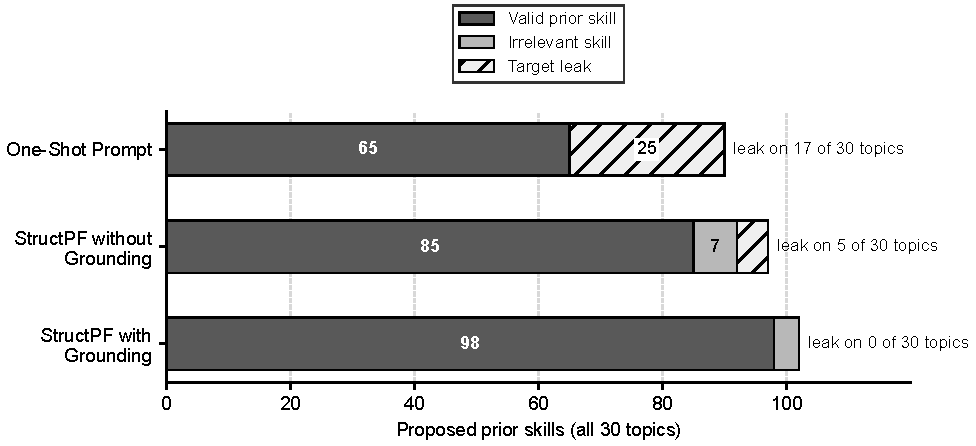
\includegraphics[width=0.9\textwidth]{figures/fig6_6_prior_knowledge_check.pdf}
    \caption[Study B Step 1: Prior-Knowledge Check by Generator]{Study~B Step~1: Prior-Knowledge Check by Generator}
    \label{fig:res-gate1}
\end{figure}

\subsection{Step 2: Method-Failure Check}
\label{subsec:res-gate2}

A correct judgment of prior knowledge does not guarantee that the task resists it. For the runs that pass Step~1, the target-blind solver and attempt judge of \textsc{PF Eval} apply only the valid proposed skills to the task numbers and sort each task into one of three outcomes.
\begin{itemize}
    \item \textbf{Familiar methods fall short and need the target.} None of the valid prior skills solves the task on its own, and trying them produces a tie, conflict, or gap that requires the target concept.
    \item \textbf{Bypassed by a familiar method.} At least one valid prior skill already reaches the right answer on the task numbers, or the task text states the target procedure directly.
    \item \textbf{Falls short for an unrelated reason.} The solver gets stuck because of missing data or inconsistent numbers rather than the mathematical gap to the target concept.
\end{itemize}

Figure~\ref{fig:res-gate2} shows that once the prior skills are valid, both \textsc{StructPF} variants make those skills fall short on roughly two thirds of their eligible runs, namely 16 of 24 ($67\%$) without grounding and 19 of 30 ($63\%$) with grounding, compared with 6 of 13 ($46\%$) for the one-shot prompt. Most of the remaining runs across all three generators are bypassed by a familiar method, while only a few fail for an unrelated reason.

\begin{figure}[!htb]
    \centering
    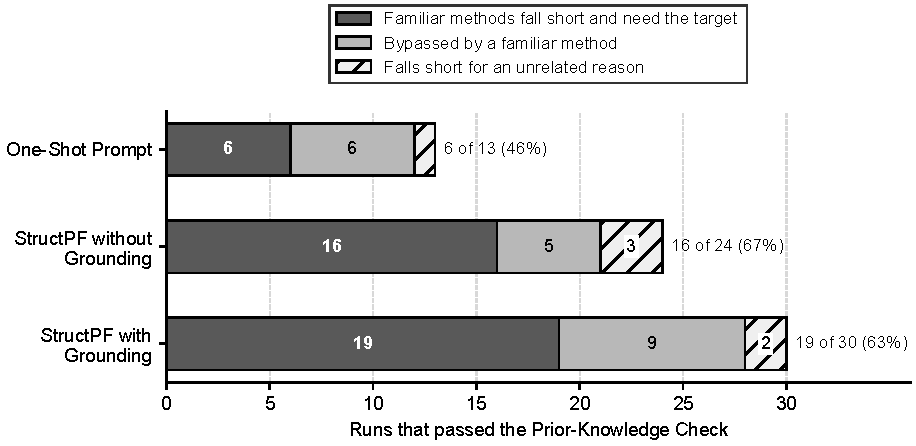
\includegraphics[width=0.9\textwidth]{figures/fig6_7_method_failure_check.pdf}
    \caption[Study B Step 2: Method-Failure Check by Generator]{Study~B Step~2: Method-Failure Check by Generator}
    \label{fig:res-gate2}
\end{figure}

Taken together, Figures~\ref{fig:res-gate1} and~\ref{fig:res-gate2} separate the contribution of each design choice in three findings.
\begin{enumerate}[leftmargin=0.6cm,label=\textbf{\arabic*.},itemsep=0.5em,topsep=0.4em]
    \item \textbf{External Curriculum Grounding Is Needed to Fix the Prior-Knowledge Boundary}\\[0.2em]
    Giving prior-knowledge identification its own stage in \textsc{StructPF} without grounding already reduces target leaks compared with one-shot prompting, because the model focuses on what students know before designing the task. However, relying on the model's own memory still leaks the target concept on several topics, and only grounding Stage~1 on the curriculum graph removes target leaks completely.
    \item \textbf{Valid Prior Knowledge Alone Is Not Enough Without Staged Task Design}\\[0.2em]
    Even when the one-shot prompt identifies valid prior skills in Step~1, more than half of its tasks are still solved directly by those familiar methods in Step~2. Planning the impasse and verifying the numbers in Stage~2 are therefore still required to make valid prior skills fall short.
    \item \textbf{Curriculum Grounding and Staged Design Work Together Across All Topics}\\[0.2em]
    \textsc{StructPF} with grounding shows a slightly lower pass rate in Step~2 only because Stage~1 grounding brings all 30 topics into Step~2, including the harder topics that already failed Step~1 without grounding. Across the full set of 30 topics, combining curriculum grounding with staged design raises the number of working PF tasks from 6 for one-shot prompting and 16 without grounding to 19 with grounding.
\end{enumerate}

\section{Negative Results with Simulated Students}
\label{sec:res-negative-signals}

While developing \textsc{StructPF} and \textsc{PF Eval}, we also tested two other ways to build and evaluate Productive Failure tasks. Both attempts produced negative results, yet they are worth reporting because they revealed important pitfalls and steered our design toward the final pipeline.

\subsection{Classroom Pathway Reproduction}
\label{subsec:res-kapur-pathways}

\textbf{Motivation}\\[0.2em]
To design a task around the mathematical structure of Productive Failure, we need to know the concrete solution and error pathways that students try before instruction so that Stage~2 can choose numbers where those attempts break down. Prior work showed that simulated students given a knowledge profile can imitate student responses in several domains~\cite{lu2024,scarlatos2025smart}, while mathematics studies warned that models often fall back on expert calculations~\cite{liu2023novice,srivatsa2025abilities}. Before relying on external curriculum data, we therefore tested whether an LLM role-playing a student can think like a student and reproduce the diverse pathways observed in a real PF classroom. If it worked, we could obtain realistic student pathways directly from the model to guide PF task generation instead of grounding Stage~1 on curriculum data.

\textbf{Setup}\\[0.2em]
To test this against real classroom ground truth, we used Kapur and Bielaczyc's Grade~7 bicycle-handover problem~\cite{kapur2012}, where the paper documents six distinct calculation strategies and error pathways produced by real student groups. We collected 24 independent attempts from simulated students across GPT-4.1 and GPT-4.1 mini under two prerequisite profiles without giving them the solution or forcing a specific error, and coded which of the six classroom pathways they actually used.

\begin{figure}[!htb]
    \centering
    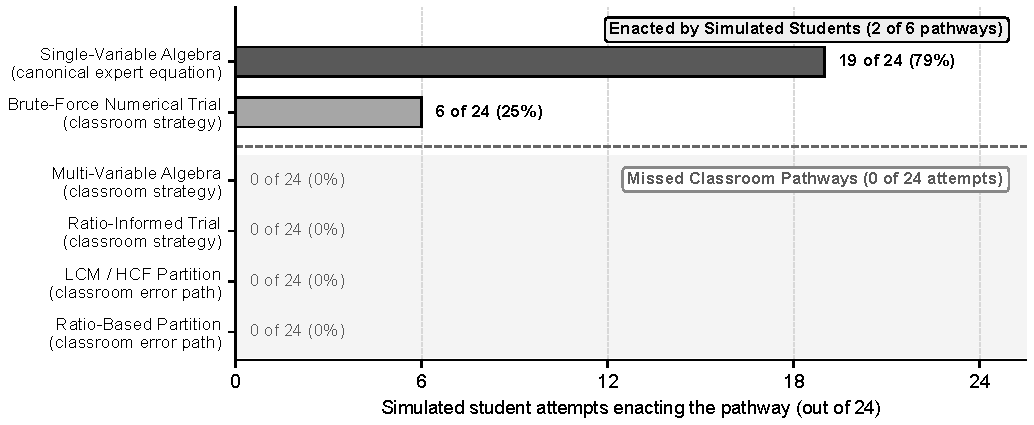
\includegraphics[width=0.88\textwidth]{figures/fig6_8_kapur_pathways.pdf}
    \caption[Kapur and Bielaczyc Classroom Pathways Enacted by Simulated Students]{Kapur and Bielaczyc~\cite{kapur2012} Classroom Pathways Enacted by Simulated Students}
    \label{fig:res-kapur-pathways}
\end{figure}

\textbf{Finding}\\[0.2em]
Figure~\ref{fig:res-kapur-pathways} shows that 19 of the 24 simulated student attempts ($79\%$) jumped straight to the canonical single-variable algebra equation and 21 of the 24 solved the problem completely, while 6 ($25\%$) tried brute-force numerical guessing. None of the 24 attempts ($0\%$) enacted the ratio-based partition or common-multiple partition error pathways that real Grade~7 groups used in the classroom, nor did any attempt draw the journey diagram documented in the paper. Because a simulated student defaults to expert algebra instead of producing the diverse student error pathways seen in real classrooms, we cannot rely on LLM-generated pathways on their own, which is why Stage~1 of \textsc{StructPF} grounds prior methods on the real-world curriculum graph instead.

\subsection{Virtual-Classroom Feedback Loop}
\label{subsec:res-virtual-classroom}

\textbf{Motivation}\\[0.2em]
Even when Stage~1 and Stage~2 use curriculum grounding, we cannot be sure how students will react to a generated task until someone attempts it. We therefore wanted to test whether a virtual classroom of simulated students could serve as an automatic refinement loop after Stage~3, where simulated student attempts are fed back into the generator to rewrite tasks that missed an intended approach.

\textbf{Setup}\\[0.2em]
Because any revision step might improve a draft simply by giving the model a second pass to polish its own work, we compared two matched revision paths across six generated tasks using the exact same revision prompt and call budget (Figure~\ref{fig:res-virtual-classroom}a). In the self-review baseline, the rewriter sees only the task text (with no simulated students), whereas in the virtual-classroom feedback loop, the rewriter receives the exact same task text plus eight simulated student attempts.

\begin{figure}[!htb]
    \centering
    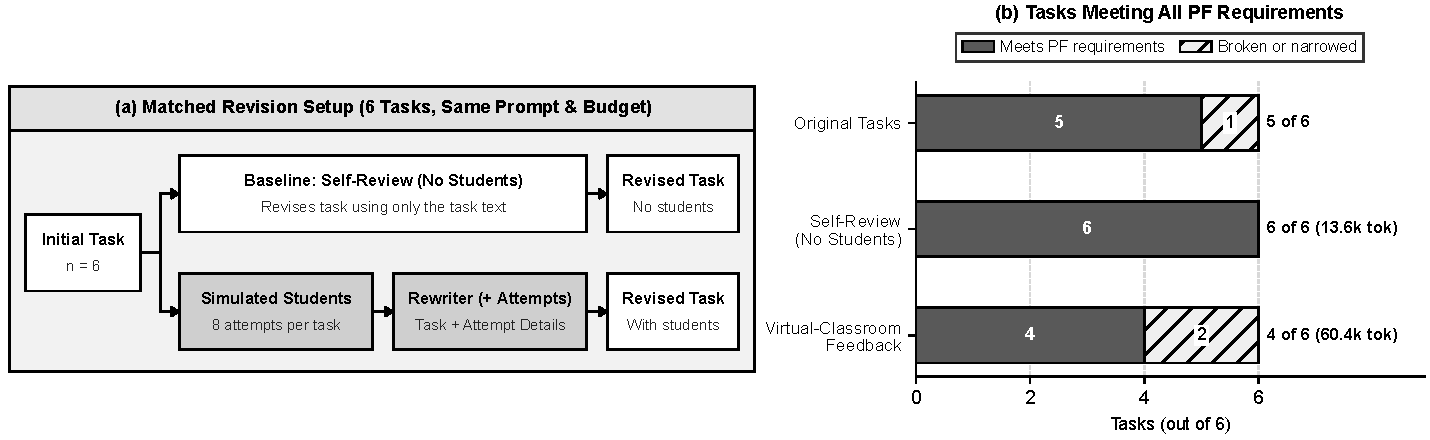
\includegraphics[width=\textwidth]{figures/fig6_9_virtual_classroom_feedback.pdf}
    \caption[Virtual-Classroom Feedback Loop versus Self-Review]{Virtual-Classroom Feedback Loop versus Self-Review}
    \label{fig:res-virtual-classroom}
\end{figure}

\textbf{Finding}\\[0.2em]
As shown in Figure~\ref{fig:res-virtual-classroom}b, adding the simulated student attempts actually reduced the number of valid PF tasks from 5 of 6 to 4 of 6 while using more than four times as many tokens ($60{,}365$ versus $13{,}572$), whereas self-review without simulated students passed all 6 of 6. Because the simulated students skipped naive shortcuts and solved the original tasks directly, their attempts made the tasks look too easy, pushing the rewriter to add extra constraints that narrowed the problem or broke its mathematical assumptions. We therefore dropped the post-Stage~3 feedback loop and evaluate tasks in \textsc{PF Eval} with a calculator-checked prior-knowledge solver instead.
